

\chapter{实验结果及分析}
对于本次实验,我们使用了 API FOX 测试 GET, HEAD 以及 404 的返回(如图\ref{fig:apifox});使用浏览器测试服务器是否顺利返回文本、图片等(如图\ref{fig:web});使用liso\_client 测试新的缓冲区管理办法(如图\ref{fig:buffer})。均通过。

\begin{figure}[htbp!]
    \centering
    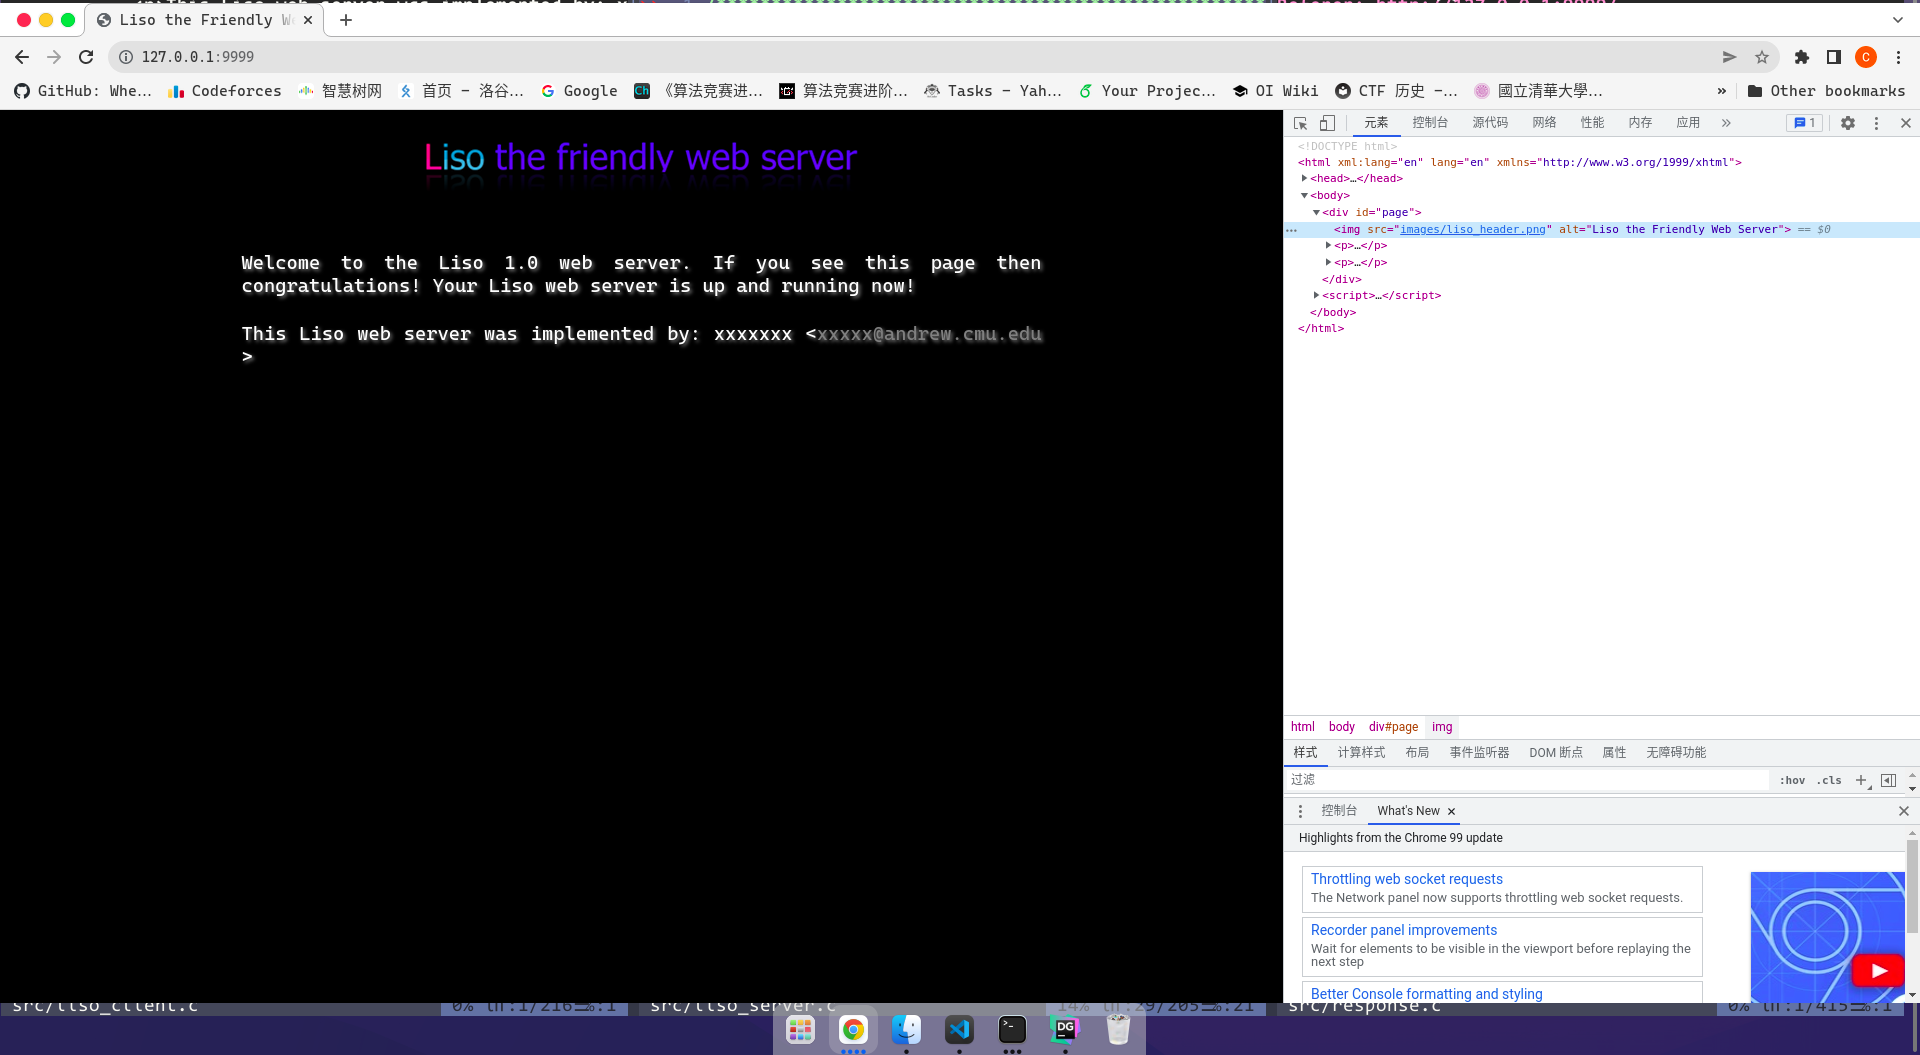
\includegraphics[width=5.5in]{liso_web.png}
    \caption{Liso Web Test}\label{fig:web}
\end{figure}

\section{任务测试点}
全部通过(如图\ref{fig:lab2autolab})。前几次因为没有正确修改文件名,所以一直 "WA0"。直到问了助教才修改名字为 liso\_server 以及 liso\_client 。
\section{结果分析}
在浏览器的测试中,发现和使用 liso\_client 测试不同,当出现有 404 的情况时,我们的 liso\_server 不会立刻进入下一轮监听,而是一直处于处理请求的情况。我们推测,是由于没实现 chunk 导致的。

\section{日志}
日志信息如图\ref{fig:logger} 所示。在日志信息里可以看到,我们的 recv 操作,每次最多接收 1025 字节的信息,单次可能不能完全接收一份报文的所有信息,但通过我们动态数组的管理,我们能够轻易完成 Pipeline 的测试。

\begin{figure}[htbp!]
    \centering
    \subfigure[Liso API FOX Test]{\label{fig:apifox}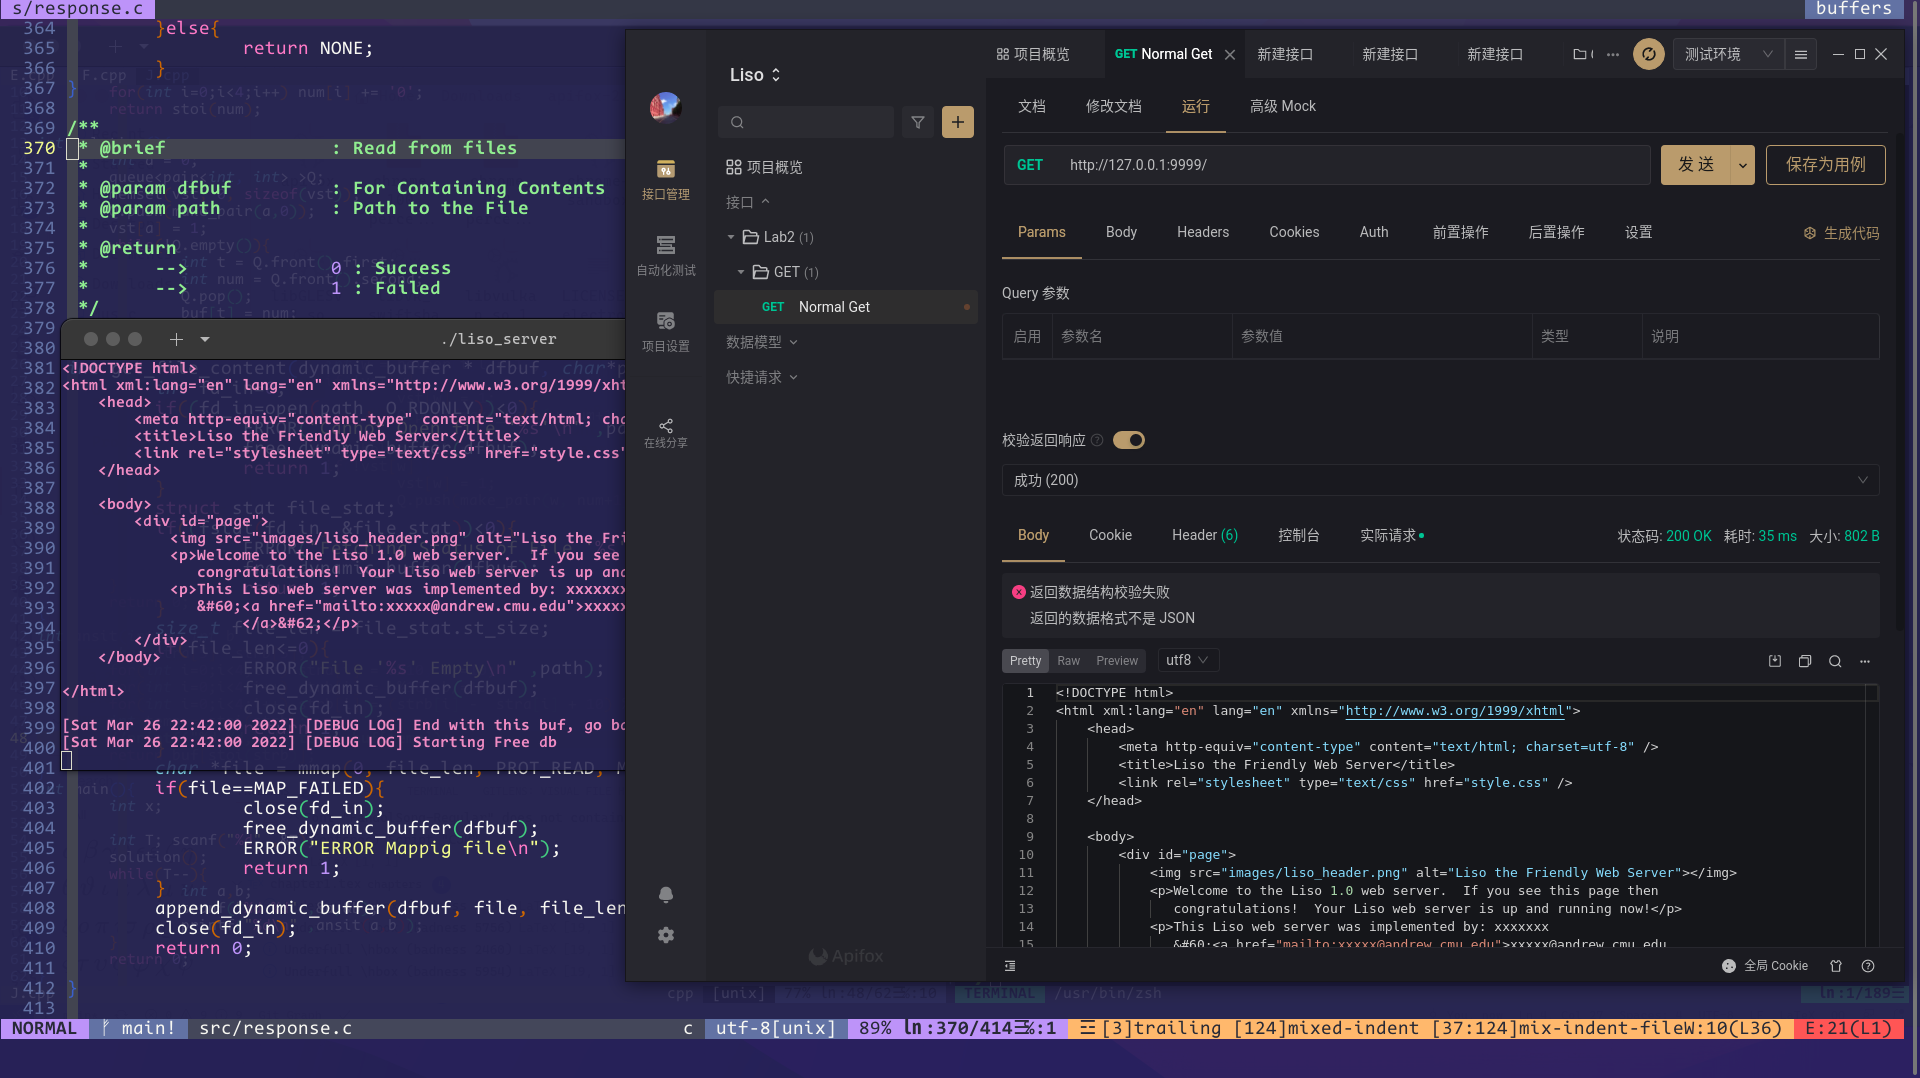
\includegraphics[width=2.75in]{APIFox_NormalGet.png}}
    \subfigure[Liso Test]{\label{fig:normal}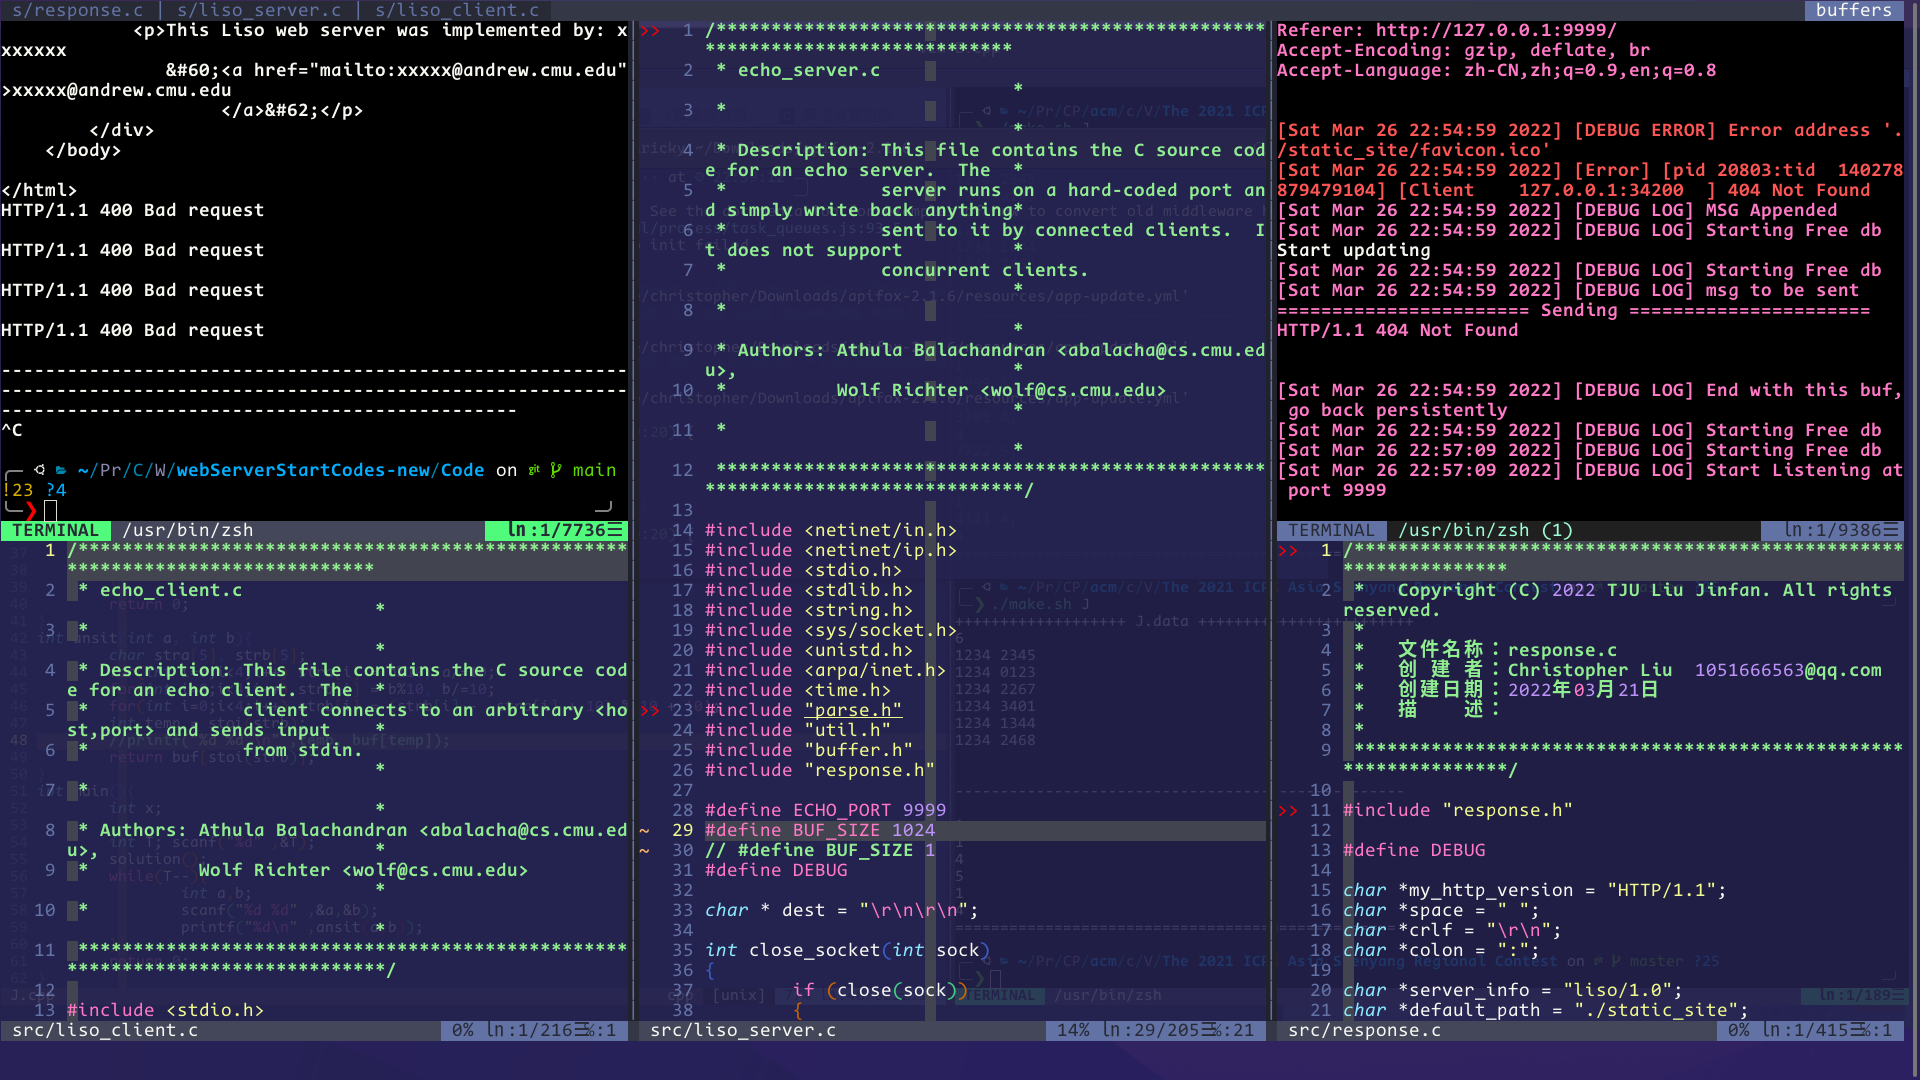
\includegraphics[width=2.75in]{liso_test.png}}

    \subfigure[部分 log 输出]{\label{fig:logger}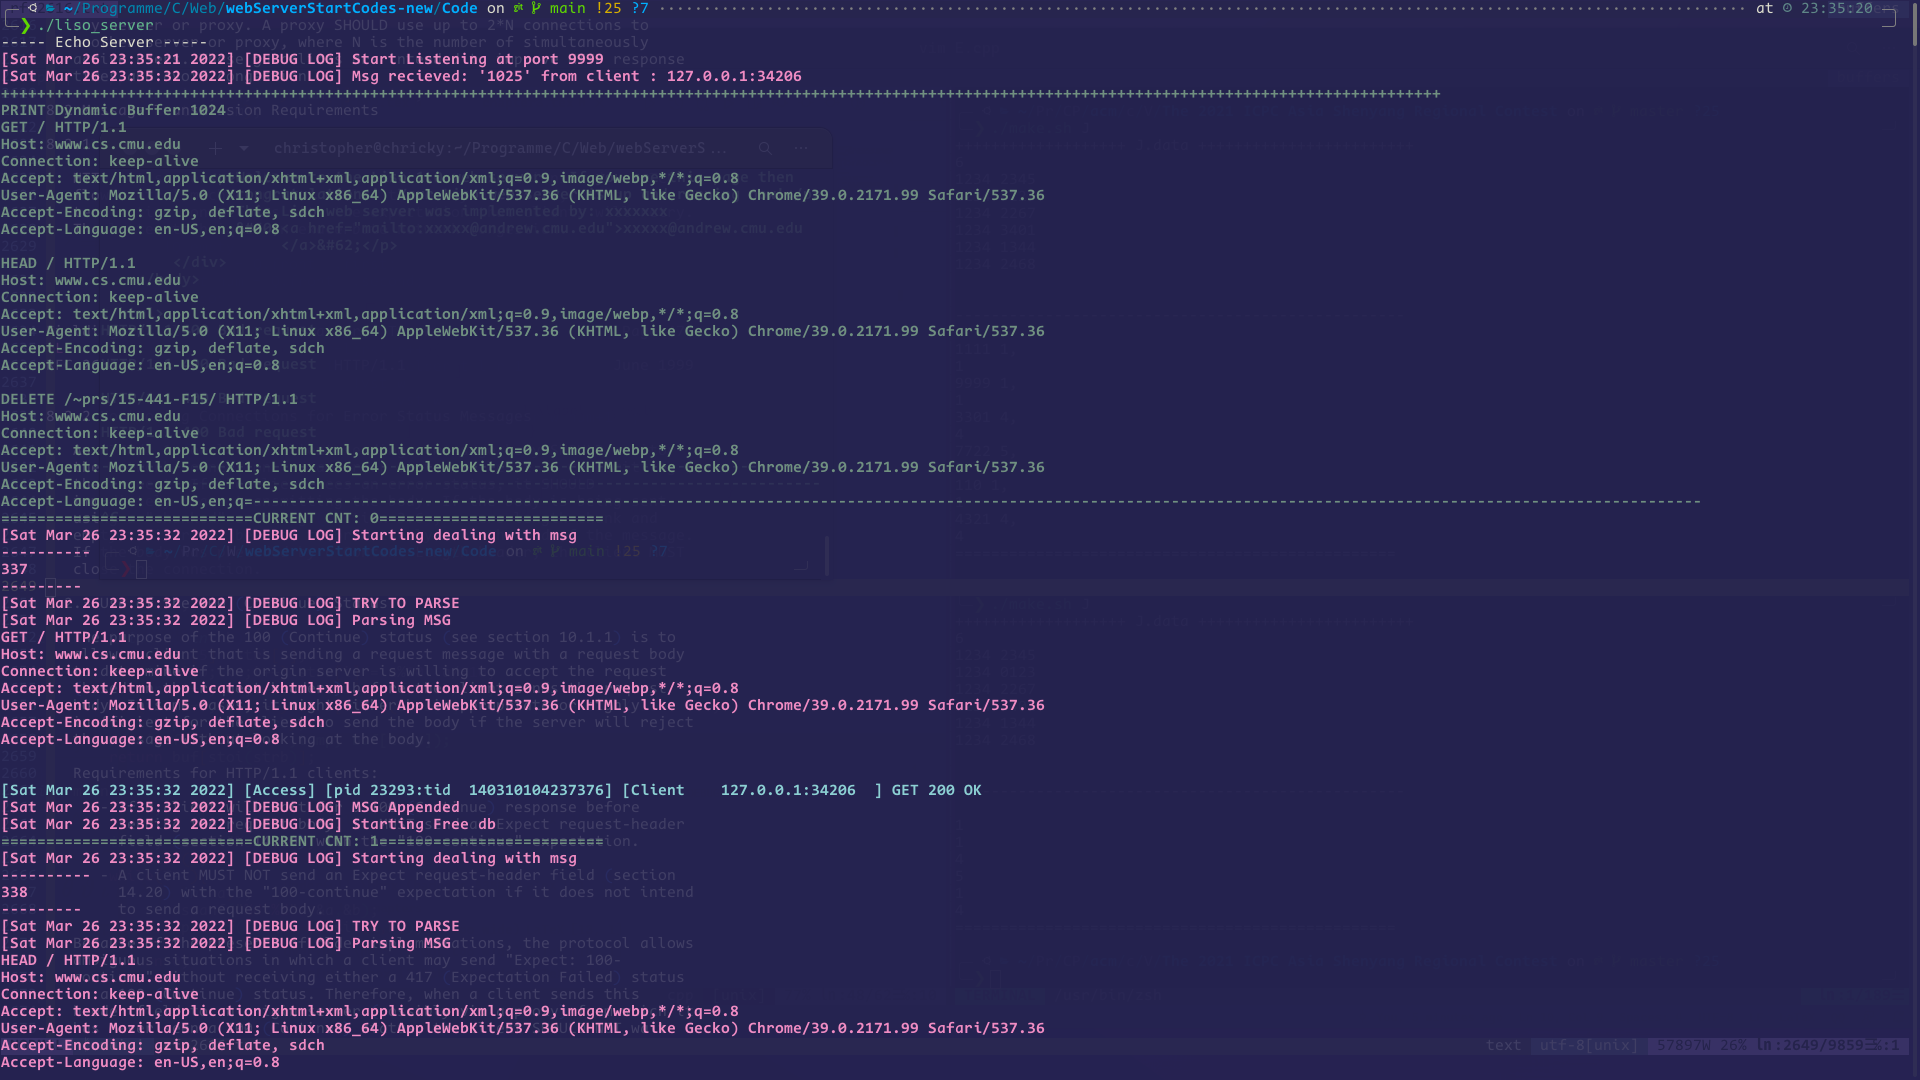
\includegraphics[width=5.5in]{lab2Logger.png}}
    \subfigure[AutoLab 测试结果]{\label{fig:lab2autolab}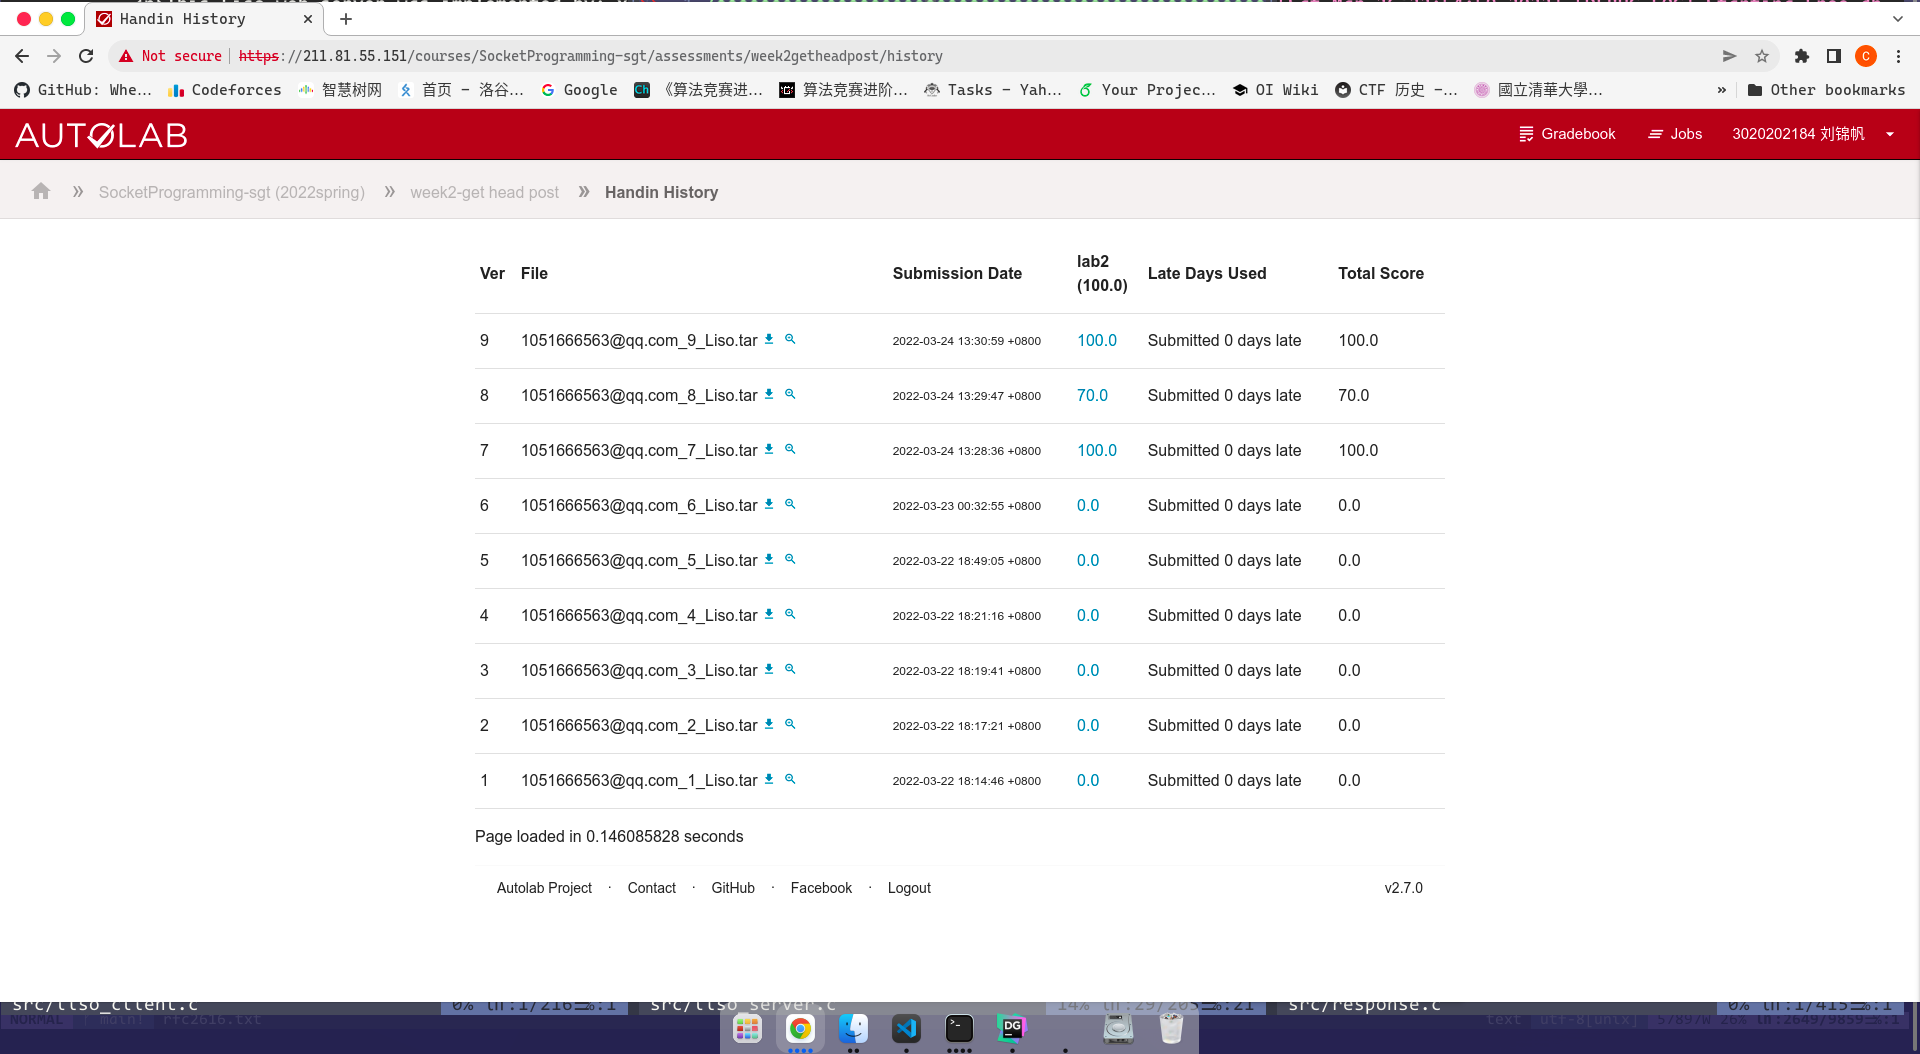
\includegraphics[width=5.5in]{lab2autolab.png}}
    \caption{测试结果展示}\label{fig:result}
\end{figure}

